%--- Começo do código ---

%Parte B
\subsection{Análise Exploratória dos Dados}

O objetivo principal da análise exploratória é compreender a estrutura interna dos dados e identificar as variáveis mais pertinentes, ou seja, quais características fisiológicas possuem maior poder discriminatório para diferenciar os três estados de estresse definidos no estudo: no stress, interruption e time pressure. Além disso, por meio da análise, é possível detectar eventuais problemas, como a redundância, antes de se proceder à modelagem. Esta etapa é crucial para garantir a robustez das etapas futuras.\\

\noindent \textbf{Visualização dos Dados}\\

Para compreender a distribuição dos preditores, cada variável foi analisada individualmente, com suas estatísticas descritivas fundamentais: a média, o desvio padrão e a assimetria calculadas. As Tabelas \ref{tab:estatisticas_part1of3}, \ref{tab:estatisticas_part2of3} e \ref{tab:estatisticas_part3of3} apresentam essas estatísticas para cada preditor do conjunto de dados, permitindo identificar a magnitude e a dispersão de cada variável fisiológica. A análise foi realizada inicialmente de maneira incondicional, ou seja, sobre o conjunto de dados completo e, posteriormente, de modo condicional, levando em consideração as classes, visando avaliar o poder discriminatório de cada variável. Além disso, para cada uma das análises, foi  utilizado histogramas para visualizar a forma de cada distribuição e boxplots para identificar outliers. A Figura \ref{fig:HR} mostra o histograma e o box-plot incondicional da variável HR, que apresenta uma leve assimetria positiva e uma maior concentração dos dados entre 65-85 bpm. 

%IMAGENS E TABELAS

\begin{table*}[!b]
\centering
\caption{Estatísticas descritivas dos preditores (Parte 1 de 3).}
\sisetup{round-mode=places, round-precision=2}
\setlength{\tabcolsep}{0pt}
\begin{tabular*}{\textwidth}{@{\extracolsep{\fill}} l S[table-format=4.2] S[table-format=4.2] S[table-format=3.2] S[table-format=2.2] S[table-format=2.2] S[table-format=1.2] S[table-format=2.2] S[table-format=1.2] S[table-format=1.2] S[table-format=1.2] S[table-format=1.2] }
\toprule
\textbf{Estatística} & {MEAN\_RR} & {MEDIAN\_RR} & {SDRR} & {RMSSD} & {SDSD} & {SDRR\_RMSSD} & {HR} & {pNN25} & {pNN50} & {KURT} & {SKEW} \\
\midrule
Média           & 846.650104 & 841.965890 & 109.352531 & 14.977498 & 14.976767 & 7.396597 & 73.941824 & 9.841143 & 0.866001 & 0.523235 & 0.041628 \\
Desvio-padrão   & 124.603984 & 132.321005 & 77.117025 & 4.120766 & 4.120768 & 5.143834 & 10.337453 & 8.195574 & 0.990189 & 1.790348 & 0.699522 \\
Assimetria      & 0.648000 & 0.925513 & 2.363789 & 0.399529 & 0.399668 & 3.707939 & 0.411721 & 1.203114 & 1.264137 & 5.722209 & 1.223005 \\
\bottomrule
\end{tabular*}
\label{tab:estatisticas_part1of3}
\end{table*}

\begin{table*}[!b]
\centering
\caption{Estatísticas descritivas dos preditores (Parte 2 de 3).}
\sisetup{round-mode=places, round-precision=2}
\setlength{\tabcolsep}{0pt}
\begin{tabular*}{\textwidth}{@{\extracolsep{\fill}} l S[table-format=1.2e-1] S[table-format=-1.2e-1] S[table-format=1.4] S[table-format=1.4] S[table-format=1.4] S[table-format=1.2] S[table-format=1.2] S[table-format=1.2] S[table-format=4.2] S[table-format=2.2] S[table-format=3.2] }
\toprule
\textbf{Estatística} & {\thead{MEAN\\\_REL\_RR}} & {\thead{MEDIAN\\\_REL\_RR}} & {\thead{SDRR\\\_REL\_RR}} & {\thead{RMSSD\\\_REL\_RR}} & {\thead{SDSD\\\_REL\_RR}} & {\thead{SDRR\_RMSSD\\\_REL\_RR}} & {\thead{KURT\\\_REL\_RR}} & {\thead{SKEW\\\_REL\_RR}} & {VLF} & {VLF\_PCT} & {LF} \\
\midrule
Média           & -0.000002 & -0.000465 & 0.018571 & 0.009701 & 0.009701 & 2.006817 & 0.523235 & 0.041628 & 2199.580170 & 64.289242 & 946.530252 \\
Desvio-padrão   & 0.000163 & 0.000868 & 0.005455 & 0.003897 & 0.003897 & 0.375845 & 1.790348 & 0.699522 & 1815.773422 & 16.774844 & 574.171780 \\
Assimetria      & 0.112796 & -0.948009 & 0.869543 & 1.258784 & 1.258784 & 0.838587 & 5.722209 & 1.223005 & 1.960735 & -0.410836 & 1.349076 \\
\bottomrule
\end{tabular*}
\label{tab:estatisticas_part2of3}
\end{table*}


\begin{table*}[!b]
\centering
\caption{Estatísticas descritivas dos preditores (Parte 3 de 3).}
\sisetup{round-mode=places, round-precision=2}
\setlength{\tabcolsep}{0pt}
\begin{tabular*}{\textwidth}{@{\extracolsep{\fill}} l S[table-format=2.2] S[table-format=-1.2] S[table-format=2.2] S[table-format=1.2] S[table-format=1.2] S[table-format=4.2] S[table-format=3.2] S[table-format=1.2] S[table-format=2.2] S[table-format=3.2] S[table-format=-1.2] S[table-format=1.2] S[table-format=1.0] }
\toprule
\textbf{Estatística} & {LF\_PCT} & {LF\_NU} & {HF} & {HF\_PCT} & {HF\_NU} & {TP} & {LF\_HF} & {HF\_LF} & {SD1} & {SD2} & {sampen} & {higuci} & {datasetId} \\
\midrule
Média           & 34.095182 & 95.566718 & 39.245603 & 1.615576 & 4.433282 & 3185.356025 & 115.977200 & 0.048506 & 10.593708 & 154.178997 & 2.062471 & 1.182292 & 2.000000 \\
Desvio-padrão   & 16.040290 & 4.123365 & 45.398869 & 1.761073 & 4.123365 & 1923.227187 & 360.855129 & 0.049238 & 2.914795 & 109.170222 & 0.206999 & 0.062192 & 0.000000 \\
Assimetria      & 0.425164 & -1.645603 & 2.476530 & 2.021882 & 1.645603 & 1.452435 & 9.781091 & 2.159372 & 0.399668 & 2.363386 & -3.091012 & 0.335008 & 0.000000 \\
\bottomrule
\end{tabular*}
\label{tab:estatisticas_part3of3}
\end{table*}

\begin{figure*}[t]
\centerline{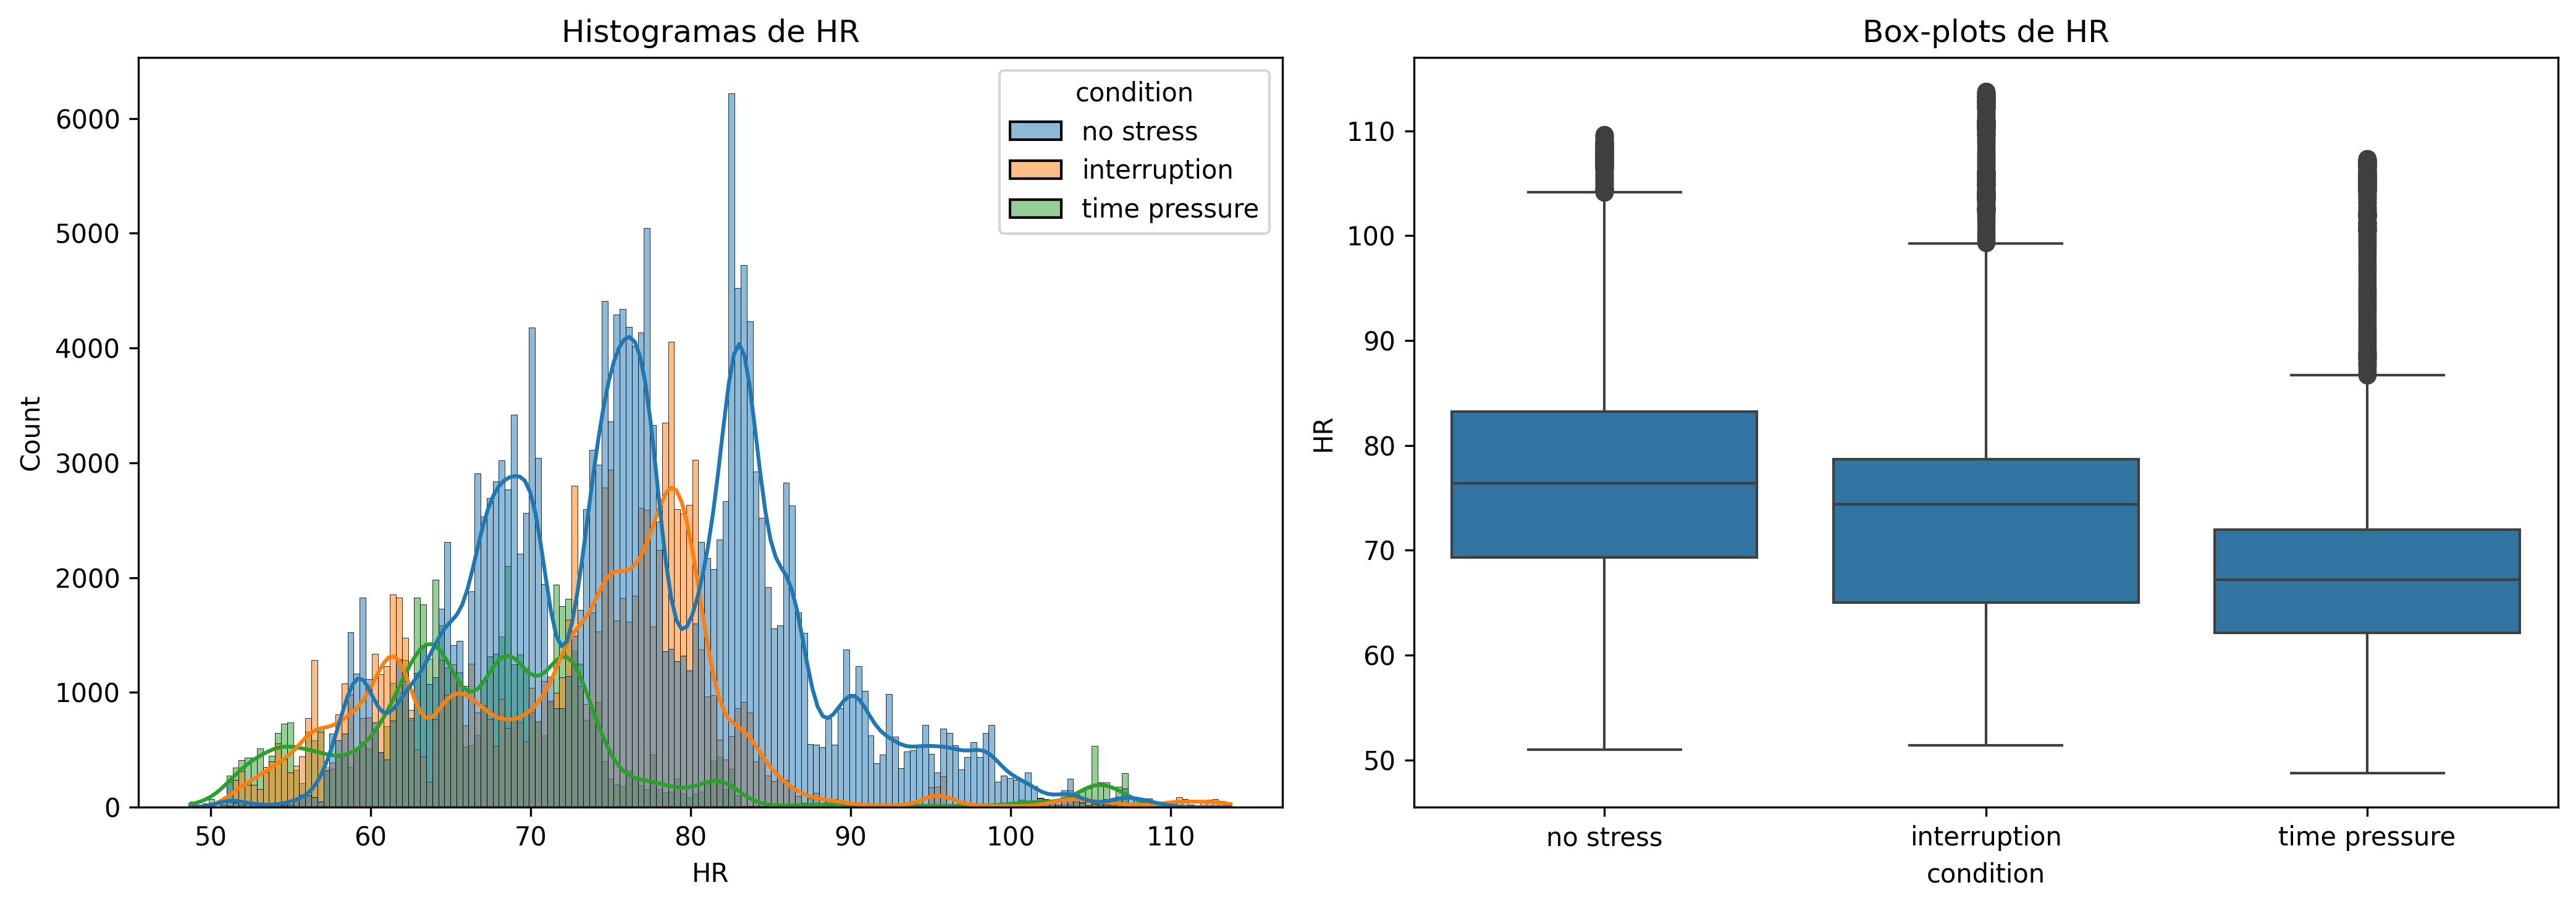
\includegraphics[width=0.7\linewidth]{imagens/HR.png}}
\caption{Histograma e box-plot incondicional de HR.}
\label{fig:HR}
\end{figure*}

\begin{figure}[htbp]
\centerline{\includegraphics[width=1\linewidth]{imagens/mean_RR.jpg}}
\caption{Histogramas de MEAN$\textunderscore$RR por classe.}
\label{fig:mean_RR}
\end{figure}


A Figura \ref{fig:mean_RR} apresenta os histogramas por classe de MEAN$\textunderscore$RR, que mostra claramente ser uma variável discriminatória, pois, dependendo da classe, temos diferentes distribuições.

A análise bivariada investigou as relações entre os pares de preditores utilizando diagramas de dispersão, com pontos coloridos conforme a classe \textit{condition}, permitindo avaliar visualmente a separação entre classes. Complementarmente, foi calculada uma matriz de correlação e visualizada como mapa de calor, facilitando a identificação de padrões de dependência linear e multicolinearidade entre os preditores.


%--- Parte C ---

%Parte D
\subsection{Análise de Componentes Principais}

A Análise de Componentes Principais (PCA) é uma técnica estatística multivariada utilizada para a redução de dimensionalidade e extração de características. Sua principal importância reside na capacidade de transformar um conjunto complexo de variáveis correlacionadas em um novo conjunto, dimensionalmente menor, de variáveis não correlacionadas, chamadas componentes principais, retendo o máximo possível da variância original dos dados. A metodologia para a sua aplicação neste trabalho seguiu os seguintes passos propostos por Kuhn e Johnson \cite{b8}:

\begin{enumerate}
    \item \textbf{Padronização dos Dados:} O processo iniciou-se com centralização na média, onde a média de cada variável é subtraída de seus valores, e o escalonamento pela variância, onde o resultado é dividido pelo desvio padrão, de forma a  assegurar que a análise se concentrasse na estrutura de variância em detrimento da localização espacial dos dados.
    \item \textbf{Cálculo da Matriz de Covariância e Decomposição em Autovalores e Autovetores:} Com os dados padronizados, foi novamente calculada uma matriz de covariância. Ela foi então decomposta para encontrar seus autovalores ($\lambda$) e autovetores ($\vec{v}$). Nesta etapa, os autovetores representam as direções dos componentes principais, enquanto os autovalores correspondentes quantificam a magnitude da variância capturada por cada autovetor.

    \item \textbf{Projeção:} Os autovetores foram, então, ordenados de forma decrescente com base em seus autovalores, com os dados sendo projetados nos dois componentes principais com os maiores autovalores (PC1 e PC2).
\end{enumerate}


%--- Resto do código ---

